\documentclass[11pt]{article}
%\documentclass[3p,review,11pt]{elsarticle}
\usepackage{lineno,hyperref,notoccite,etoolbox}
\modulolinenumbers[5]
\usepackage[margin=1in]{geometry}

\makeatletter
\def\ps@pprintTitle{%
	\let\@oddhead\@empty
	\let\@evenhead\@empty
	\def\@oddfoot{\centerline{\thepage}}%
	\let\@evenfoot\@oddfoot}
\makeatother
\usepackage{setspace}
\singlespacing
\usepackage{mathptmx}
\usepackage{float,wrapfig}

\usepackage{sectsty}
\sectionfont{\fontsize{12}{12}\selectfont}
\newcommand{\vs}{\vspace{2mm}}
\usepackage{array}
\usepackage{multicol,graphicx}
%\renewcommand{\baselinestretch}{2} 

\begin{document}

\begin{center}
\textbf{Understanding and Mitigating Uranium Nitride Corrosion for Use in Nuclear Reactors} \par \vs
Ember Sikorski  \
\end{center}
\rule{6.5in}{0.1mm} \\
\vs
\textbf{Abstract} \\
Before uranium nitride (UN) can be implemented as an accident tolerant fuel, its instability in air must be addressed. This review surveys current research on the degradation of UN pellets, powders, and films caused by oxygen or water. Experimental studies suggest that nitriding surfaces and adding intermetallic phases may improve uranium nitride performance. Computational studies show atomistically stable configurations of adsorbates at uranium nitride surfaces. The differences in reported UN corrosion products and avenues for mitigating corrosion are discussed.
\\
\rule{6.5in}{0.1mm}	
\vs

\begin{multicols}{2}


\section{Introduction}
%introduce topic
%highlight importance of topic to nuclear power production
%materials it affects
%components of the reactor involved

Uranium nitride (UN) is considered a prospective fuel for both light water reactors (LWRs) and Generation IV reactors \cite{Streit2005,Mizutani1998}. The higher fissile density of UN as compared to uranium dioxide benefits fast reactors due to the lower neutron cross section \cite{Silva2009}. This higher actinide density additionally benefits LWRs because UN pellets can remain in the reactor longer, leading to longer time between shut downs, and reducing money lost \cite{Lopes2017}. For all reactor types, the high thermal conductivity and high melting temperature make UN an optimal material to mitigate accidents \cite{Lopes2017}.
\par 
While nuclear power initially developed uranium dioxide for the fuel pellet, the call for accident tolerant fuels (ATF) after Fukushima has drawn attention back to nitrides \cite{Johnson2016}. However, ATF materials must maintain current operational standards as well as improve safety \cite{Zinkle2014}. Despite the beneficial properties of UN, it is unstable in the presence of steam or even air \cite{Lopes2017,Johnson2016,Jolkkonen2017}. In the event of cladding failure in a LWR, the pellet will come into contact with steam. As UN degrades, fission products will be released from the fuel matrix, free to interact with the containment structure. Furthermore, nitrogen can react with the steam to form explosive ammonium nitrate \cite{Jolkkonen2017}.
\par 
 In the case of Generation IV reactors, most designs use alternative coolants. However, the instability of UN in air hinders fabrication into a fuel pellet \cite{Lopes2017}. Short of solving UN corrosion at high temperatures and pressures for LWRs, corrosion in air must be mitigated for use as a Generation IV fuel.
 \par 
 To assess the current state of UN corrosion research, this review examines seven studies from within the past decade. The first two studies were designed to better understand UN oxidation in the presence of oxygen \cite{Liu2013} and steam \cite{Jolkkonen2017}. In the next study, Johnson et al. \cite{Johnson2016} studied oxidation rates of UN as compared to other prospective fuels.  Lu et al. \cite{Lu2016} and Lopes et al. \cite{Lopes2017} each investigated a method to mitigate UN corrosion: nitriding and introduction of an intermetallic phase, respectively. The last two studies used computational modeling to probe the atomistic initiation of UN corrosion by studying oxygen \cite{Bocharov2013} and water \cite{Bo2016} at UN surfaces. In the discussion, the discrepancies and drawbacks of the studies, possible solutions, and the prospect of UN as a fuel are examined.

\section{Review}
%current efforts in the area
%may include research on demonstration of issue or mitigation strategies


\par 
The UN corrosion mechanism was first proposed as \cite{Dell1967,Sugihara1969}:
\begin{equation}
\mbox{UN} + 2\mbox{H}_{2}\mbox{O} \rightarrow \mbox{UO}_{2} + \mbox{NH}_{3} + \frac{1}{2} \mbox{H}_{2} \quad ,
\end{equation}
with an intermediary step of: 
\begin{equation}
3\mbox{UN}+2\mbox{H}_{2}\mbox{O} \rightarrow \mbox{UO}_{2}+\mbox{U}_{2}\mbox{N}_{3}+2\mbox{H}_{2} \quad .
\end{equation}

To better understand UN corrosion, Jolkkonen et al. \cite{Jolkkonen2017} subjected UN pellets to superheated steam. The authors tried varied densities of UN pellets, ranging from 77.6\% to 97.7\% of theoretical density. Jolkkonen et al. found no NO or NO$_{2}$ was produced. Additionally, even after hydrolysis finished, residual N$_{2}$ was found in the resultant powder. The lowest density pellet resulted in the greatest amount of degradation, yielding rapid H$_{2}$ production followed by a significant release of N$_{2}$, contrasting the other pellets which gave off N almost exclusively as NH$_{3}$. The denser pellets could last up to 90 minutes while subjected to 300 $^{\circ}$C steam, but degraded as the temperature was increased to 400 $^{\circ}$C. The pellets showed different mechanical fracture modes, with the lowest density pellets turning to powder and the higher density pellets cracking into fragments. This fragmentation would further accelerate corrosion as additional surface area is exposed.
\par 

Liu et al \cite{Liu2013} nitrided depleted $\alpha$-U by surface glow plasma nitriding (SGPN) and by plasma immersion ion implantation (PIII). After adding oxygen gas under ultra high vacuum (UHV), the SGPN prepared UN oxidized to U$_{2}$N$_{3}$ and O diffused into the uranium nitride. They proposed this mechanism as:
\begin{equation}
2\mbox{U}_{2}\mbox{N}_{3} +x \mbox{O}_{2} \rightarrow 2\mbox{U}_{2}\mbox{N}_{3}\mbox{O}_{x} \quad .
\end{equation}

In contrast, the PIII prepared UN formed UO$_{2+x}$ and off-gassed NO, described as:
\begin{equation}
2\mbox{UO}_{2}\mbox{N}_{x} + x\mbox{O}_{2} \rightarrow 2 \mbox{UO}_{2} + 2x\mbox{NO} \quad .
\end{equation}
The authors described their final products left in air as UO$_{2}$ and U$_{2}$N$_{3}$.
\par 
Johnson et al. \cite{Johnson2016} turned their focus from the mechanism to a comparison of time until oxidation between UN, uranium silicide, and uranium dioxide powders. The powders were ramped to 800$^{\circ}$C while the mass was measured with thermogravimetry. At 4.4\% open porosity, UN oxidized at 320 $^{\circ}$C, determined by 5\% mass increase. On the other hand, 0.0\% open porosity UN performed better than even UO$_{2}$, with oxidation onsets of 440 $^{\circ}$C and 405 $^{\circ}$C, respectively. The UN-10\%U$_{3}$Si$_{2}$ powder performed nearly the same as the low porosity UN, with a slightly higher oxidation onset temperature of 450$^{\circ}$C but also slightly higher mass increase due to oxide formation. The authors concluded that while using U$_{3}$Si$_{2}$ in conjunction with UN may improve fabrication of UN, it does not necessarily reduce corrosion.
\par 
 While Johnson et al. studied UN powders, Lopes et al. \cite{Lopes2017}  fabricated full pellets of UN and UN-10\%U$_{3}$Si$_{2}$. In order to reach the high densities sufficient to reduce oxidation, UN must be sintered at over 2000 $^{\circ}$C. However, this results in accelerated grain growth, creating fast diffusion pathways for both oxygen to enter and fission products to escape. To reduce this necessary temperature, an intermetallic phase of U$_{3}$Si$_{2}$ can be added during sintering.
\par 
Lopes et al. placed the pellets in an autoclave, heated to 300 $^{\circ}$C, and added 9 MPa steam. Like Jolkkonen et al. and Johnson et al., the authors found reduced reactivity with reduced porosity. They found degradation increased in time, and suggested the mechanism depended on the OH and NH$_{3}$ formed during the reaction. The oxygen formed a non-protective layer as part of a ``sandwich structure" of UO$_{2}$, U$_{2}$N$_{3}$, and UN. The larger grains were easily fragmented due to mechanical instability.

 Instead of studying bulk UN for fuel applications, Lu et al. \cite{Lu2016} examined UN films towards determining if N could reduce the reactivity of U during storage.  Films of UN$_{x}$ were prepared at stoichiometries of $x$ = 0.23, 0.68, and 1.66. Their results suggested the formation of an oxynitride, OU$_{x}$N$_{y}$, phase rather than UO$_{2}$ in the UN$_{1.66}$ film. This film formed the thinnest oxide layer, suggesting the greatest resistance to corrosion. The authors reasoned that the poor oxidation resistance of the UN$_{0.68}$ film may be due to the ease with which oxygen can fill a nitrogen vacancy in UN.
\par 
Density functional theory (DFT) has been used in several studies to probe the atomistic UN corrosion mechanism, notably by the groups Bocharov et al. \cite{Bocharov2013} and Bo et al. \cite{Bo2016}. Bocharov studied oxygen atoms and nitrogen vacancies at the UN (100) and (110) surfaces along with a tilt grain boundary. Bocharov et al. found that an N vacancy can form preferentially at the (110) surface followed by the grain boundary and then the (100) surface, but the oxygen prefered to enter at the grain boundary vacancy site. Regardless, oxygen incorporation yielded negative energy for each case. The study ended with a proposed oxidation mechanism of \cite{Bocharov2013}: 
	(1) chemisorption of O$_{2}$,
	(2) dissociation of adsorbed O$_{2}$,
	(3) adsorption of O atop U atoms,
	(4) high mobility of O along the surface, and
	(5) incorporation of O at N vacancies.
\par 
Finally, Bo et al. \cite{Bo2016} extended examination of UN to the surface in the presence of water. Using the (100) surface, Bo et al. studied water coverages ranging from one to four molecules (0.25 to 1 monolayer coverage). They reported the adsorption energies for molecular, partially dissociated, and fully dissociated water, with partially and fully dissociated water being equally favorable. After adsorption, the authors deconstructed the energy levels using local density of states, shown in \textbf{Fig. 1}. By separately plotting the hydrogen atoms as H1 and H2, they discussed the bonding between the adsorbate atoms. For instance, \textbf{Fig. 1(a)} showed the OH bond due to overlapping orbitals of O and H2 around -7.5 eV. Likewise, the increased amount of overlap between H1 and H2 in \textbf{Fig. 1(b)} compared to \textbf{Fig. 1(a)} indicated a stronger hybridization.
\begin{center}
	%\caption{}
	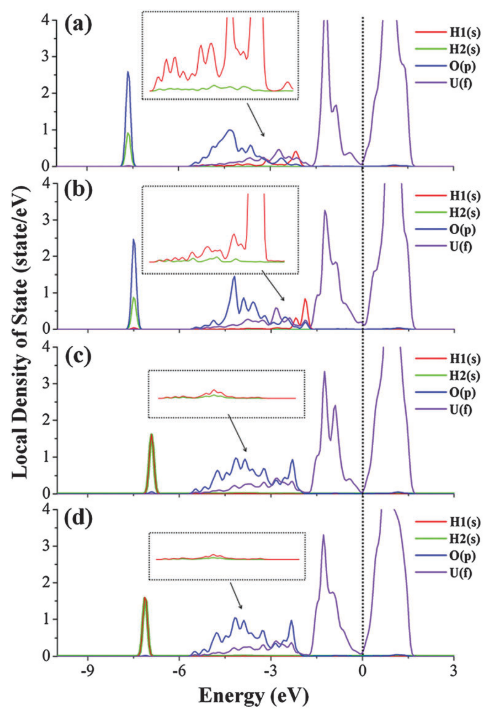
\includegraphics[height=8cm]{Bo} \\	
\end{center}
\textbf{Fig. 1.} Local density of states for four different H$_{2}$O and H$_{2}$ adsorption configurations on UN (001) surface. The dashed line represents the Fermi level \cite{Bo2016}.

%what they reported, later talk about how this is useless
\begin{table*}[!t]
	
	\setlength{\extrarowheight}{1.5mm}
	\begin{tabular}{ p{3.5cm} p{5cm} p{2.5cm} p{2.5cm}  }
		
		\multicolumn{4}{c}{\textbf{Table 1.} Select experimental parameters from studies of UN degradation in oxygen or steam.} \\
		\hline
		& Starting Material &Temperature & Pressure\\
		\hline
		Jolkkonen et al. \cite{Jolkkonen2017}   &  UN pellets (77 - 97\%TD) &400 - 425 $^{\circ}$C&  0.05 MPa \\
		Johnson et al. \cite{Johnson2016}   & UN powder ($\approx$20 mg)     &800 $^{\circ}$C&  not reported \\
		Lu et al. \cite{Lu2016}  & UN films    &20 $^{\circ}$C&   UHV \\
		Lopes et al. \cite{Lopes2017}   & UN pellets (95 - 99 \% TD)    & 300 $^{\circ}$C&   9 MPa \\
		Liu et al. \cite{Liu2013}& nitrided U & not reported  & UHV\\
		\hline
	\end{tabular}
\end{table*}
\section{Discussion}

\par Across the studies, the experiments differed by starting material, processing of starting material, experimental methods, and reported products. To better illustrate the differences in experimental parameters, select variables are given in \textbf{Table 1}. In regards to reported products, one can see that the formation of N$_{2}$ and residual N reported by Jolkkonen et al. \cite{Jolkkonen2017} directly opposes mechanism (1). Similarly, Liu et al. \cite{Liu2013} reported U$_{2}$N$_{3}$ as a final product, while the first proposed mechanism describes it as only an intermediary (\textbf{Eq. 2}). Jolkkonen et al. report no NO production while Liu et al. include NO in the mechanism (\textbf{Eq. 4}) of conversion of oxyntitride to uranium dioxide. Lopes et al. and Lu et al. both reported an oxide layer, but Lopes et al. described it as a "sandwich" of UO$_{2}$, U$_{2}$N$_{3}$, and UN while Lu et al. described it as UN$_{x}$O$_{y}$.
%move to review section
 The results are highly specific to experimental parameters; Lu et al. demonstrated that whether a UO$_{2}$ or  OU$_{x}$N$_{y}$ oxide forms depends on the N concentration, and Jolkkonen et al. showed the products depended on porosity. With this variance in methods and products, it is impossible to draft a conclusive corrosion mechanism from the current literature. To determine the mechanism experimentally, studies will have to be conducted that vary only one parameter from \textbf{Table 1} at a time, e.g. starting material, temperature, or pressure.
%experiments need to hold more variables constant - describe table
%while other computational methods are available, corrosion is a chemical problem and mechanical codes such as FEA or even mesoscale models (phase field) will not help. Quantum mechanical treatment is required to 
%M D codes require already knowing the interaction potential, and the very problem here is that we don't know how they will interact

\par With DFT, it is possible to precisely control the experimental parameters without requiring acquisition of new equipment. However, studies thus far have focused on very low oxygen and water coverages. During a real-life accident scenario, it is very unlikely that a pristine surface will encounter a single O atom or water molecule. While such results may be useful for feeding into larger scale models that rely on these values for validation, such UN models have yet to be created and published. Furthermore, the discussed DFT studies reported only ideal adsorption sites, defect formation energies, orbital overlap, etc. Such data cannot be straightforwardly converted into a reaction mechanism. While Bocharov et al. \cite{Bocharov2013} did propose a mechanism, the description was given based on single atom or molecule motion and did not describe the formation of intermediaries or products.

One option to simulate a more dynamic reaction mechanism would be to use a molecular dynamics (MD) model. MD can model thousands of atoms compared to DFT which is limited to approximately one hundred atoms. MD also includes temperature effects, unlike DFT, which are integral to nuclear systems. However, this increase in scale and temperature consideration comes at the sacrifice of quantum mechanical accuracy, as MD uses Newtonian mechanics. Thus, MD is incapable of modeling an evolving relationship between elements, such as the difference between a U atom in UN interacting with an O atom and a U atom in UN$_{x}$O$_{y}$ interacting with an O atom. To gain the benefits of the scale of MD and the quantum mechanical treatment of DFT, it is possible to use the \textit{Ab initio} molecular dynamics (AIMD) method. This method quantum mechanically calculates interactions on-the-fly, but evolves the system using Newton's second law instead of the gradient of the interaction energy. 
%new discussion of DFT - expand on need for multiple studies 
%if they present a mechanism, is this the only mechanism? are there competing
%reactions?
\par 
To obtain information relevant to determining a UN corrosion mechanism, future computational efforts will require examination of greater oxygen and water concentrations and a survey of relevant temperatures and pressures. Due to the computational cost of DFT, AIMD offers a more optimal path towards determining the UN corrosion mechanism through simulation.
%studies so far have focused on adsorption sites and single atom movement,
%instead of mechanistic behavior: what are the product species? what are the 
%intermediaries required to reach the product?
%talk about AIMD
%Bocharov gives very initial mechanism - no reveal to intermediaries, doesn't utilize spontaneous structures from DFT
\par In spite of the lack of a definite mechanism, Lopes et al. \cite{Lopes2017} have demonstrated that U$_{3}$Si$_{2}$ can improve UN sinterability. Similarly, Lu et al. \cite{Lu2016} have shown that nitriding a uranium surface can reduce the thickness of the formed oxide layer.
Mitigating UN corrosion will likely come from a combination of increasing density, nitriding, and adding intermetallics or dopants. First, studies have agreed on the benefit of creating a low porosity pellet to reduce reactivity \cite{Lopes2017,Johnson2016,Jolkkonen2017}. Second, nitrided pellets may resist corrosion, but if the pellet cracks it will be just as susceptible to degradation as pure UN pellets. Third, intermetallics improve ease of sintering, but whether they do or do not mitigate corrosion remains under debate. An as-of-yet unstudied dopant may prove to mitigate corrosion in the event of cracking more successfully than an intermetallic. If UN can at least be made stable in air, it can be used in Generation IV reactors which use He gas for coolant. However, for Generation IV reactors using liquid salts, metal, or even water at higher core temperatures, extensive studies will be needed to understand how UN will interact with a new coolant or starting from higher temperatures during an accident.
\par 
If UN can be implemented as a fuel, its higher thermal conductivity will result in a temperature at the centerline closer to that at the surface, ideally leading to more uniform pellet expansion and reduced contact with the cladding. If the pressure between cladding and fuel can be reduced, failure of the cladding can be delayed and response time in the event of an accident increased. The nitrides, silicides, or other dopants added to the fuel will need to be accounted for in terms of neutronics, such that the use of control rods can properly be adjusted.

\par 


%\end{multicols}

%\begin{multicols}{2}

\section{Summary}
%reiterate highlights
The high actinide density, high thermal conductivity, and high melting temperature of UN make it a prospective fuel for accident tolerance in LWRs and for use in Generation IV reactors. However, its chemical instability in an atmosphere of oxygen and water have hindered its implementation. 
\par Jolkkonen et al. \cite{Jolkkonen2017} studied UN pellets under superheated steam to better understand the UN corrosion mechanism. They found better corrosion resistance from denser pellets and residual N even after complete oxidation. Liu et al. \cite{Liu2013} used two different methods to create UN and found one method produces oxynitride while the other produces uranium dioxide. Johnson et al. \cite{Johnson2016} found UN-U$_{3}$Si$_{2}$ powder oxidized at approximately the same rate as pure, dense UN powder. Lopes et al. \cite{Lopes2017} also found denser pellets reacted less with steam and found grain size contributed to corrosion mechanically. Lu et al. showed higher stoichiometry UN films exhibited thinner oxide layers. Bocharov et al. \cite{Bocharov2013} showed the favorability of oxide incorporation at a nitrogen vacancy and proposed an atomistic reaction mechanism. Lastly, Bo et al. \cite{Bo2016} showed favorable dissociated water adsorption.
\par The experiments give insight into how the corrosion reaction changes with respect to experimental parameters, though the exact corrosion mechanism remains elusive. Experimental studies should work towards holding more variables constant, so that the cause of differences in resultant products can be determined explicitly. Computational studies have begun to look at single adsorption mechanisms and future studies should investigate larger adsorbate coverages, as well as pressure and temperature. 
\par 
UN corrosion issues may be solved through increasing density, nitriding, and the addition of dopants or intermetallics. If fully realized as a fuel, UN may reduce the severity of accidents and lead to higher burn up. The change in neutron economy caused by adjusting UN will need to be carefully considered before implementation in a reactor.




\bibliography{nuclear}
\bibliographystyle{elsarticle-num}


\end{multicols}
\end{document}  